\documentclass{beamer}

\mode<presentation> {
  \usetheme{PaloAlto}
  \usecolortheme{default}
  \usefonttheme{default}
  \setbeamertemplate{navigation symbols}{}
  \setbeamertemplate{caption}[numbered]
}

\usepackage{polski}
\usepackage[utf8x]{inputenc}
\usepackage{hyperref}
\usepackage{color}
\usepackage{listings}
\usepackage{pgfpages}
\pgfpagesuselayout{resize to}[physical paper width=8in, physical paper height=6in]

\title[Git]{Git - system kontroli wersji}
\author{Piotr Kowalski}
\institute{Wyższa Szkoła Informatyki Stosowanej i Zarządzania}
\date{24-05-2013}

% ------------------------------------------------------------------------------

\begin{document}
\lstdefinestyle{customc}{
  belowcaptionskip=1\baselineskip,
  breaklines=true,
  frame=L,
  xleftmargin=\parindent,
  language=C,
  showstringspaces=false,
  basicstyle=\footnotesize\ttfamily,
  keywordstyle=\bfseries\color{green!40!black},
  commentstyle=\itshape\color{purple!40!black},
  identifierstyle=\color{blue},
  stringstyle=\color{orange},
}

\lstdefinestyle{customasm}{
  belowcaptionskip=1\baselineskip,
  frame=L,
  xleftmargin=\parindent,
  language=[x86masm]Assembler,
  basicstyle=\footnotesize\ttfamily,
  commentstyle=\itshape\color{purple!40!black},
}

\lstset{escapechar=@,style=customc}
	
% --------------------------------------

\begin{frame}
  \titlepage
\end{frame}

% --------------------------------------

\section{Wprowadzenie}

\begin{frame}{Wprowadzenie}
\begin{itemize}
  \item Co to jest system kontroli wersji?
  \item Dlaczego \texttt{git} jest zdobył serca programistów?
\end{itemize}
\vskip 1cm
\begin{block}{System kontroli wersji}
Oprogramowanie służące do śledzenia zmian głównie w kodzie źródłowym oraz pomocy programistom w łączeniu zmian dokonanych przez wiele osób w różnych momentach.
\end{block}
\end{frame}

% --------------------------------------

\section{Rodzina systemów}

\begin{frame}{Scentralizowane}
\begin{itemize}
  \item RCS
  \item CVS
  \item Subversion
  \item GNU CSSC, klon SCCS
  \item JEDI VCS
\end{itemize}
\end{frame}

\begin{frame}{Rozproszone}
\begin{itemize}
  \item Bazaar
  \item Codeville
  \item Darcs
  \item Git
  \item GNU Arch
  \item Mercurial
  \item Monotone
  \item svk
\end{itemize}
\end{frame}

\begin{frame}{Zamknięte (własnościowe) systemy kontroli wersji}
\begin{itemize}
  \item BitKeeper firmy BitMover
  \item Code Co-op firmy Reliable Software
  \item Perforce firmy Perforce Software
  \item Rational ClearCase firmy IBM
  \item Sablime firmy Lucent Technologies
  \item StarTeam firmy Borland
  \item Visual SourceSafe firmy Microsoft
  \item Visual Studio Team Foundation Server firmy Microsoft
\end{itemize}
\end{frame}

\begin{frame}{Historia}
\begin{itemize}
	\item Prace nad Gitem rozpoczęły się po tym, jak BitKeeper, używany wtedy do rozwoju Linuksa, przestał być darmowy dla projektów o otwartym kodzie źródłowym. 
\vskip 1cm
	\item Prace nad Gitem rozpoczęły się 3 kwietnia 2005 roku, projekt został ogłoszony 6 kwietnia, 7 kwietnia Git obsługiwał kontrolę wersji swojego własnego kodu, 18 kwietnia pierwszy raz wykonano łączenie kilku gałęzi kodu, 27 kwietnia Git został przetestowany pod względem szybkości z wynikiem 6,7 łat na sekundę, a 16 czerwca Linux 2.6.12 był hostowany przez Gita.
\end{itemize}
\end{frame}

\begin{frame}{Założenia}
Torvalds szukał rozproszonego systemu kontroli wersji, który mógłby być użyty zamiast BitKeepera, głównymi kryteriami wyboru były:
\begin{itemize}
	\item Wziąć przykład z CVS, czego nie robić.
	\item System powinien być rozproszony.
	\item System powinien być chroniony przed błędami w repozytorium (przypadkowymi, jak awaria twardego dysku, jak i złośliwymi, wprowadzonymi przez kogoś).
	\item System powinien być szybki.
	\item Pierwsze dwa punkty wyeliminowały wszystko prócz Monotone'a, a czwarty punkt wyeliminował wszystko, więc Torvalds postanowił napisać własny system kontroli wersji.
\end{itemize}
\end{frame}

\begin{frame}{Cele}
\end{frame}

% --------------------------------------

\section{Składowe}

\begin{frame}{Branch}
\end{frame}

\begin{frame}{Tag}
\end{frame}

% --------------------------------------

\section{Git w życiu codziennym}

\subsection{GitHub}

\begin{frame}{GitHub - rejestracja}
	\begin{figure}
	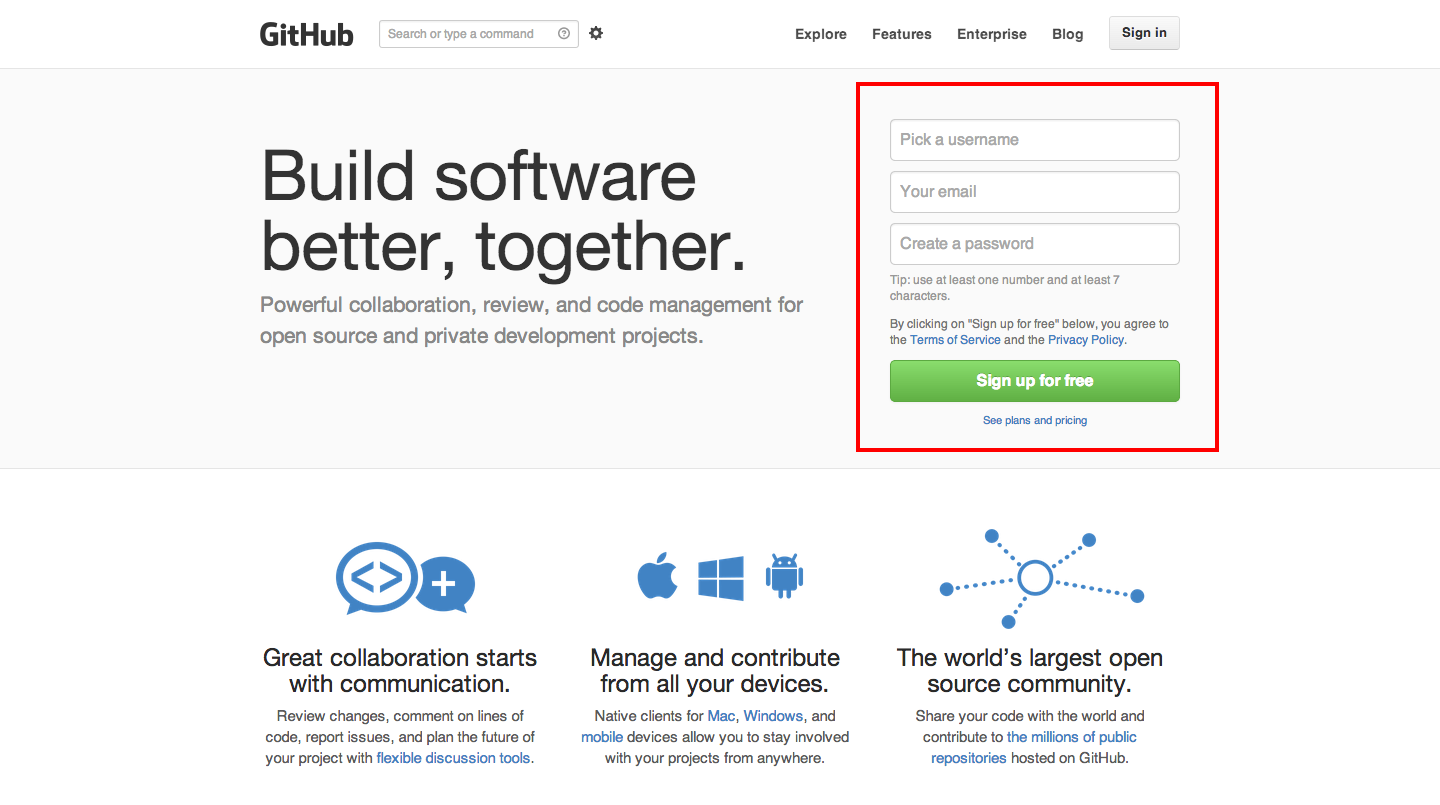
\includegraphics[width=\textwidth]{sign-up.png}
	\caption{\label{fig:sign-up}Rejestracja konta}
	\end{figure}
\end{frame}

\begin{frame}{GitHub - logowanie}
	\begin{figure}
	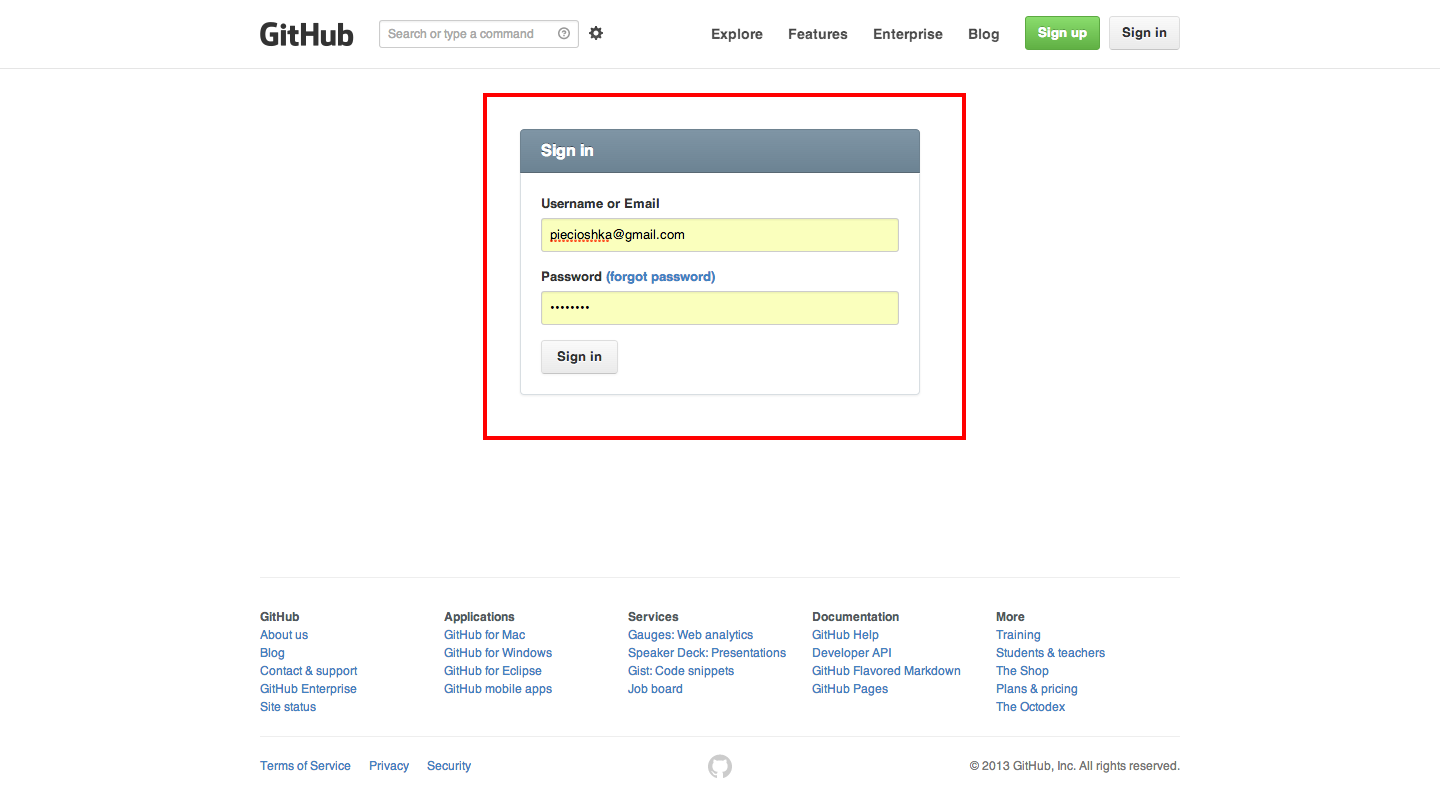
\includegraphics[width=\textwidth]{sign-in.png}
	\caption{\label{fig:sign-in}Logowanie użytkownika}
	\end{figure}
\end{frame}

\begin{frame}{GitHub - tworzenie nowego repozytorium}
	\begin{figure}
	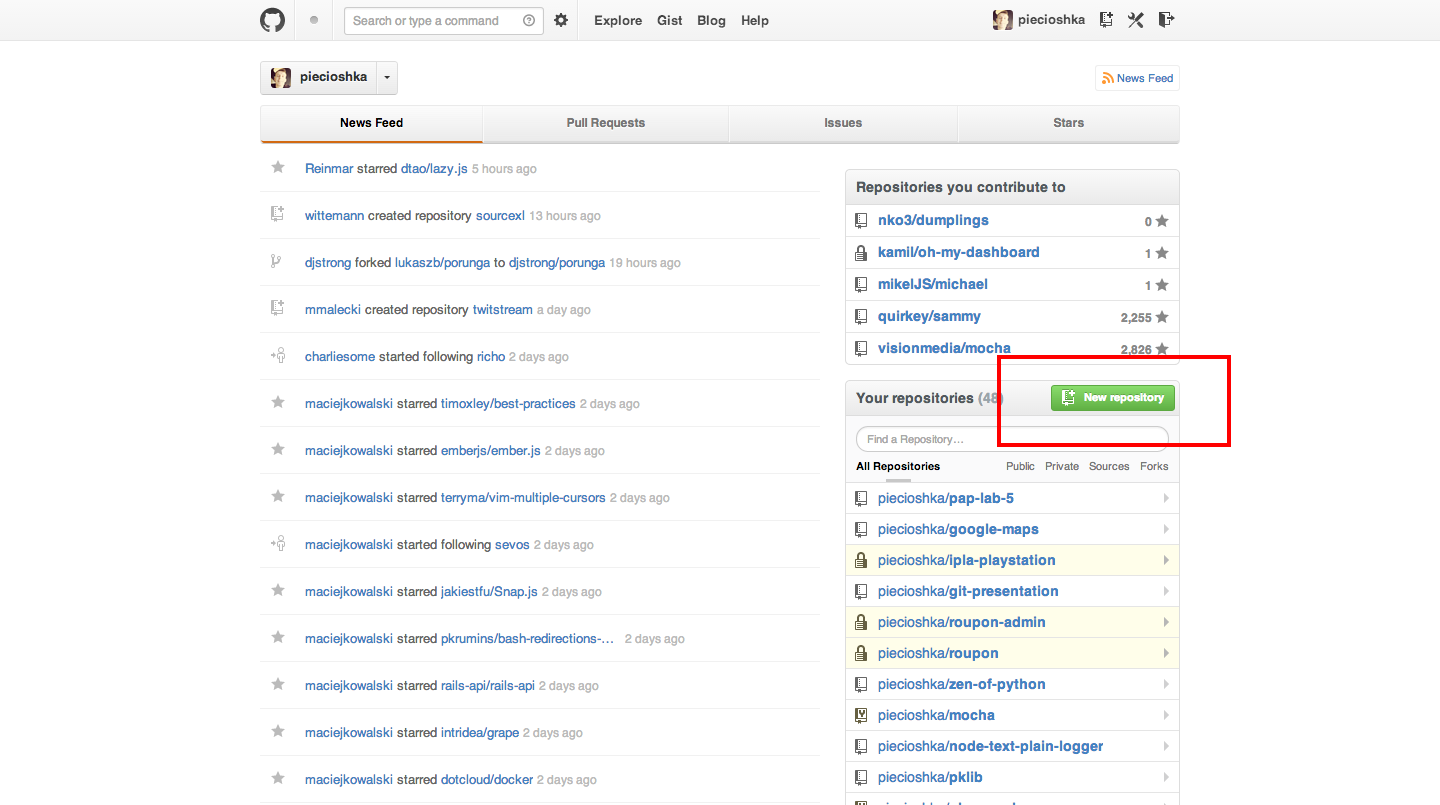
\includegraphics[width=\textwidth]{create-repo-link.png}
	\caption{\label{fig:create-repo-link}Link do tworzenia nowego repozytorium}
	\end{figure}
\end{frame}

\begin{frame}{GitHub - nowe repozytorium}
	\begin{figure}
	\includegraphics[width=\textwidth]{new-repo.png}
	\caption{\label{fig:new-repo}Nowe repozytorium}
	\end{figure}
\end{frame}

\begin{frame}{GitHub - nowe puste repozytorium}
	\begin{figure}
	\includegraphics[width=\textwidth]{new-repo-settings.png}
	\caption{\label{fig:new-repo-settings}Ustawienia repozytorium}
	\end{figure}
\end{frame}

\begin{frame}{Pierwszy projekt}


	
	\begin{lstlisting}[frame=single]
	    struct listNode {
	    dataType data;
	    listNode *next;
	    };
		
	\it \$ mkdir test
	\it \$ touch README.md
	\it \$ git init
	\it \$ git add README.md
	\it \$ git commit -m "first commit"
	\it \$ git remote add origin git@github.com:piecioshka/test.git
	\it \$ git push -u origin master
	    \end{lstlisting}
\end{frame}

\begin{frame}{Praca lokalna}
\end{frame}

\begin{frame}{Praca zdalna}
\end{frame}

% --------------------------------------

\section{Podsumowanie}

\begin{frame}{Podsumowanie}
\end{frame}

\begin{frame}{Linki}
\begin{itemize}
  \item \url{http://git-scm.com/book/pl/Pierwsze-kroki-Wprowadzenie-do-kontroli-wersji}
  \item \url{https://github.com/piecioshka/git-presentation}
\end{itemize}
\end{frame}

\end{document}
